
%(BEGIN_QUESTION)
% Copyright 2010, Tony R. Kuphaldt, released under the Creative Commons Attribution License (v 1.0)
% This means you may do almost anything with this work of mine, so long as you give me proper credit

Suppose we have an Allen-Bradley model ``SLC 500'' PLC connected to a limit switch, a hand switch, and a motor contactor as shown in this illustration:

$$\includegraphics[width=15.5cm]{i04532x01.eps}$$

Unfortunately, the motor is not starting up when it should.  You are summoned to investigate, so you connect a laptop PC to the PLC to examine the ``live'' status of the program elements:

$$\includegraphics[width=15.5cm]{i04532x02.eps}$$

Based on your examination of this program, explain why the motor is not starting.

\underbar{file i04532}
%(END_QUESTION)





%(BEGIN_ANSWER)

The contactor is not energizing because the PLC ``thinks'' the hand switch is in the ``disable'' position.  I'll let you figure out what type of wiring or component fault might cause this.

%(END_ANSWER)





%(BEGIN_NOTES)

The contactor is not energizing because the PLC ``thinks'' the hand switch is in the ``disable'' position.  Possible faults include the following:

\begin{itemize}
\item{} The hand switch is actually in the ``disable'' position
\item{} Enable/disable switch contacts failed shorted
\item{} PLC input card channel {\tt IN2} failed (bit always reading high)
\item{} Bit {\tt I:3/2} forced to a value of 1
\end{itemize}











\vfil \eject

\noindent
{\bf Prep Quiz:}

$$\includegraphics[width=15.5cm]{i04532x01.eps}$$

An operator tells you that the contactor in this system is not energizing, when it should be energizing.  You immediately go to the failed system and connect a laptop PC to examine the ``live'' program display.  From this information, determine a wiring fault that could account for why the contactor is not energizing when it should:

$$\includegraphics[width=15.5cm]{i04532x03.eps}$$












\vfil \eject

\noindent
{\bf Prep Quiz:}

$$\includegraphics[width=15.5cm]{i04532x01.eps}$$

An operator tells you that the contactor in this system is not energizing, when it should be energizing.  You immediately go to the failed system and connect a laptop PC to examine the ``live'' program display.  From this information, determine a wiring fault that could account for why the contactor is not energizing when it should:

$$\includegraphics[width=15.5cm]{i04532x04.eps}$$

%INDEX% PLC, relating I/O status to virtual elements

%(END_NOTES)


